\documentclass[a4paper]{jarticle}

\usepackage[dvipdfmx]{graphicx}

%\input{macro}

\topmargin -28mm
\oddsidemargin -15mm
\evensidemargin -15mm
\textwidth 185mm
\textheight 275mm
\columnsep 6mm

\def\zenjitu{平成30年2月15日}
\def\toujitu{平成30年2月16日}
\def\zenjituyoubi{{\zenjitu}(木)}
\def\toujituyoubi{{\toujitu}(金)}
\def\busuu{26}
\def\room{情報科学研究科B棟1階B101}
% \Eps{filename}{caption}{label}{scale}
%\newcommand{\Eps}[4]{ \begin{figure}[hbtp] \begin{center} \psbox[scale=#4]{#1} \end{center} \vspace{-8mm} \caption{#2} \label{#3} \end{figure} }

\makeatletter
\def\section{\@startsection{section}{2}{\z@}{.8ex plus .8ex minus
.2ex}{.05ex plus .07ex}{\large\bf}}
\makeatother
\makeatletter
\def\subsection{\@startsection{subsection}{2}{\z@}{.8ex plus .8ex minus
.2ex}{.05ex plus .07ex}{\bf}}
\makeatother


\pagestyle{empty}

\begin{document}

\baselineskip 4.75mm
%行間の指定をここで行う

\twocolumn
[
\footnotesize 
\begin{center}
{大阪大学大学院情報科学研究科 マルチメディア工学専攻 博士前期課程修士学位論文発表会資料
\hfill \toujitu}\\
\medskip
{\large
{\bf Alloyにおける時相論理の記述法とWebの安全性解析手法への応用}\\
}
\medskip
{\large
        島本 隼人(セキュリティ工学講座)
}
\end{center}
]

\section{はじめに}
ウェブには漏れの無い安全性が求められるため、その解析に形式手法が用いられる。
形式手法による解析にはシステムの仕様などを数学的に記述したセキュリティモデルが必要であり、その状態変化を表すために時相論理が主に用いられる。
しかし、既存モデル\cite{BasedModel, CookieModel}ではこの時相論理の表現が不十分であり、一般的なウェブのふるまいを十分に解析できない。
この問題は、既存モデルの実装に用いられているモデル検証ツールAlloyAnalyzerで利用する言語が時相論理の表現を持たないことに起因する。
したがって、本研究ではAlloyAnalyzerで利用可能な時相論理の記述法を考案し、これを用いてモデルの拡張と実装を行う。

\section{既存モデルにおける時相論理と問題点}
本研究では以下の2つのモデルの時相論理の表現能力の問題点を取り上げる。

まず、Akhaweらによる基礎モデル\cite{BasedModel}では時間軸を実装し、リクエストやレスポンスといったイベントの発生順序を表現可能とした。
これにより、イベントによって生じるウェブの状態変化を解析することが可能となる。

しかし、基礎モデルで包括するウェブの要素は少なく実用的ではないため、基礎モデルを拡張したCookieを包括したモデル\cite{CookieModel}(以下「Cookieモデル」とする)が提案された。
このCookieモデルでは実装済みの時間軸を応用し、イベントによって生じるCookieの状態変化を表現可能とした。
ただし、Cookieモデルの時相論理では対応するリクエストとレスポンス間での状態変化のみ表現可能であり、3状態以上の状態遷移の表現は不可能である。
この制限は、イベントが複数発生することが一般であるウェブの表現には適さないため拡張を要する。

\begin{figure}[b]
\centering
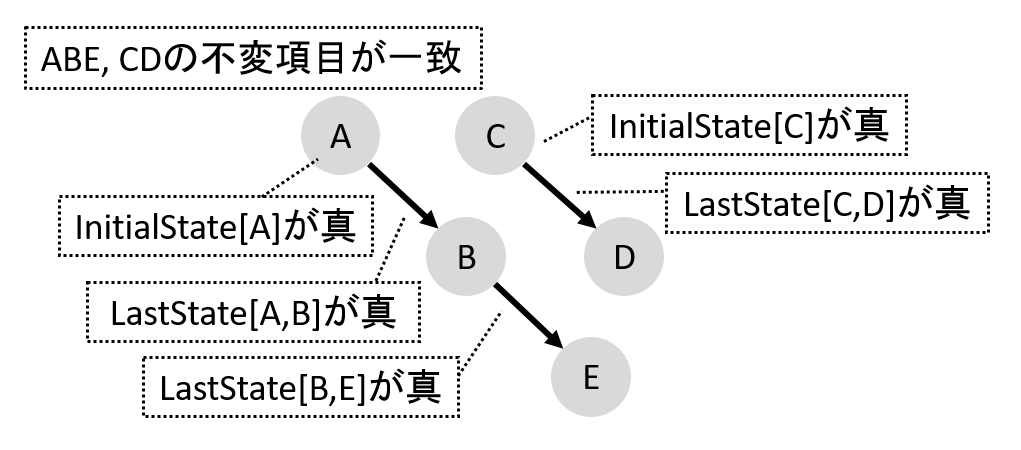
\includegraphics[width=\hsize]{./resume1.eps}
\caption{提案記述法による状態変化の表現}
\label{fig1}
\end{figure}

%\vspace{-0.2cm}
\section{時相論理の提案記述法}
本研究で提案する記述法によって、「イベントによって生じるウェブの要素の状態変化」を表現可能とする。
ここで、提案記述法はモデルの今後の更なる拡張を想定し、Cookieに限らず様々なウェブの要素に対応できる形式としている。

提案記述法による状態変化の表現方法は大きく2つに分けて考えることができ、まずはある時点でのウェブの要素の状態を表すクラスのフォーマットを作成する。
そして、これに従って表現された状態の時系列順序を表現可能とする述語を作成する。

\subsection{状態クラスのフォーマット}
表現するウェブの要素に対して、その状態クラスでは以下の項目を設定する。\\
\textbf{変化項目: }状態遷移による変化を表現したい要素\\
\textbf{不変項目: }状態遷移によって変化しない要素。複数の状態遷 移が並列に存在する場合に、各状態の不変項目の比較によ り同一の遷移であるかの判定を可能にする

\subsection{時系列を表現する述語}
上記の状態クラスに利用可能な二つの述語を作成する。
これら2つの述語を繰り返し利用することで、初期状態から帰納的に状態遷移を表現できる(図\ref{fig1})。\\
\textbf{直前の状態を判定する述語: }\\
 ある2状態A,Bが与えられた際に、AとBが同一遷移で あり、かつ、AがBの直前の状態である場合に真となる\\
\textbf{初期状態を判定する述語: }\\
 ある状態が与えられた場合に、その状態が状態遷移の初期 状態である場合に真となる

\section{記述法を用いた拡張モデル}
提案記述法を用いてキャッシュを包括するモデルを実装し、事例研究によってモデルの表現能力を評価する。

まず、フォーマットに従いキャッシュの状態を表すクラスを定義する。
ここで、キャッシュの状態変化は「あるキャッシュにおける格納レスポンスの変化」と表せるので、変化項目は「格納レスポンスの集合」、不変項目は「キャッシュ」となる。
%ここで、変化項目は「格納レスポンスの集合」、不変項目は「キャッシュ」となる。
また、レスポンスの格納といったキャッシュの動作は、前状態から起こりうる変化で全て表現できる。
例として、レスポンスの格納は「レスポンス時のキャッシュ状態は、前状態の格納レスポンスの集合にそのレスポンスを加える」と表現可能である。

このようにして実装した拡張モデルについて、キャッシュの基本的な動作に加え、既知の攻撃法を用いて事例研究を行った。
まず、キャッシュの基本的な格納や再利用といった各動作が表現できていることから、キャッシュの動作を表現できることを確認した。
また、既知の攻撃法としてBrowser Cache Poisoning Attack、Cross-site Request Forgery、Web Cache Deceptionを取り上げる
。
これらはキャッシュを利用しており、かつ、攻撃フローに3状態以上の状態遷移を含む。
結果としてこれらの攻撃法を表現できたことから、拡張モデルの時相論理が攻撃の解析に十分効果があることを確認した。

\begin{thebibliography}{9}
%\setlength{¥itemsep}{-0.5zh}
\bibitem{BasedModel} D. Akhawe et al., Towards a Formal Foundation of Web Security, \textit{Proc. of CSF'10}, pp.290-304, 2010.
\bibitem{CookieModel} P. D. Ryck et al., Automatic and Precise Client-Side Protection against CSRF Attacks, \textit{Proc. of ESORICS'11}, pp.100-116, 2011.
\end{thebibliography}

\end{document}
